% Chapter Template

\chapter{Theory} % Main chapter title
This chapter focuses on explaining the theory behind the model and the methods used in this work.
Details regarding model adjustments and how the methods were implemented are given in
\hyperref[chap:methodology]{Chapter \ref*{chap:methodology} - Methodology}.

\label{chap:theory} % Change X to a consecutive number; for referencing this chapter elsewhere, use \ref{ChapterX}


%----------------------------------------------------------------------------------------
%	SECTION 1
%----------------------------------------------------------------------------------------
\section{Background of computational disease modeling}
A common goal for disease modeling is to predict the spreading of a disease in a given population. Different approaches can be made to
achieve this goal. In 2019 Akhtar et al. presented a model based on a neural network that tries to predict the spread of the Zika virus\cite{akhatar2019dynamic}.
Models like this are promising but usually have the disadvantage of requiring big sets of data in order to train the neural network in the first place.
%(\textcolor{red}{check article if this is actually the case!}) % note
Other models are probabilistic in nature and try to predict the spreading of disease by simulating an individuals chance of contracting a
disease at any given point in time\cite{nakamura2017efficient,nakamura2020improved}. These models rely on high population numbers to compensate for errors that are caused by the random nature.
In addition, simulating the infection chances and events of each individual in such a population often requires considerable computational resources\cite{nakamura2017efficient}.
A third method of computational disease modeling is based on differential equations. This type of modeling tries to establish and express relations between different
properties of a system. In a model this could be expressed as an increase in infection rate based on the population density of a modeled region or a
change in population mobility based on the average number of cars owned per household. The challenging aspect of this method is the design and
optimization of the model itself and its equations since real life phenomena tend to be influenced by many
different factors. An increase in population mobility could be influenced by a high density of personal transportation, holiday seasons, cultural backgrounds and so on. 
his means that the relations between many
different ``moving parts'' in a system need to be identified, related to one another and then modeled and tuned correctly to make accurate predictions
of future events. However, if this modeling attempt is successful, it not only serves as a solid base for predictions of future events, it also provides insight
into the interconnected nature of a system.


%----------------------------------------------------------------------------------------
%	SECTION 2
%----------------------------------------------------------------------------------------
\section{Compartmental modeling techniques}
Compartmental modeling techniques are often used to systematically describe real-world phenomena,
like disease spreading, via differential equations\cite{kermack1991contribution,skendall1956deterministic}. In these models, the population is divided into different groups. 
Members the system can transition from one group to another. This movement is defined by the previously mentioned differential equations, that are used to model the real
world dynamics of each group. Notable examples fro compartmental modeling techniques are the ``SIR'' and the ``SEIRD'' models, which will be discussed in
the following sections. The latter of the two models was used in this work.


%-----------------------------------
%	SUBSECTION 1
%-----------------------------------
\subsection{Differential equations}
\textcolor{red}{add citations}\\ %note
%\textcolor{red}{kinda shit, add more information, starting condition, etc.}\\ %note
To understand the previously mentioned models, we will first introduce the concept of differential equations.
Differential equations are functions which contain derivatives of unknown functions, which in turn depend
on either one or more independent variables. Depending on the number of independent variables, the differential
equations are either considered \I{Ordinary Differential Equations} (ODE) or
\I{Partial Differential Equations} (PDE). The former having only a independent variable, the latter having multiple variables.
An example for each type of equation is given below, where equation \ref*{eq:ODE_ex} shows a simple ODE, and equation \ref*{eq:PDE_ex} shows a
simple PDE.\newline

\begin{align}
	\frac{\delta u}{\delta x} + b = c \label{eq:ODE_ex}\\
	\frac{\delta u}{\delta x} + \frac{\delta u}{\delta y} \cdot \frac{\delta^2 u}{\delta z^2} = c \label{eq:PDE_ex}
\end{align}

Differential equations are often used to describe the rate of change in a varying quantity in relation to another
varying quantity. This makes them very useful for describing complex biological, physical, mechanical, economic
or other scientific systems, where multiple system parameters interact with each other. However, while differential
equations are a powerful tool in describing dynamic systems, it is often difficult to find their solution (if such
a solution even exists). Solving a differential equation describes the act of finding a definition of the
unknown functions, which satisfies both the differential equation and possible other starting conditions.


%-----------------------------------
%	SUBSECTION 2
%-----------------------------------
\subsection{The SIR model}
\label{sec:SIR}
In 1927 Kermack and McKendrick\cite{kermack1991contributions} first introduced their method of mathematically describing  
the epidemiological behavior of an infectious disease. The model divides a population into three distinct groups.

\begin{enumerate}[label=$\bullet$]
	\item \B{Susceptibles (S)}: Number of Individuals that are not immune to the infection.
		%If in contact with the virus these individuals can migrate to the\linebreak ``Infected'' group
	\item \B{Infected (I)}: Number of Individuals that are currently infected with the disease.
		%Infected individuals contribute to the infection of members of the susceptible group.
		%At some point during their infection, these members transition to the ``Removed'' group.
	\item \B{Removed (R)}: Number of Individuals that  have either overcome an infection and are now immune or have succumb to the disease.
		%and are diseased. They do not spread the virus and cannot be infected again.
\end{enumerate}


Population changes in all three groups are described as ordinary differential equations.
Members of \B{S} can transition to \B{I}. This transition rate is expressed in the
form of variable $\alpha$, which is a positive, real number. This parameter includes various epidemiologically relevant factors like
population density, infectiousness, hygiene measures and many more and tries to condense them into one single value.
Transition events also occurs from \B{I} to \B{R}. This change is expressed by the variable 
$\beta$, which is a positive constant between 0 and 1. $\beta$ can be rewritten as $\frac{1}{b}$, where $b$ is the average
duration an infected individual remains contagious before it either recovers or dies. The concept of the SIR model is
illustrated in \hyperref[fig:SIR]{Figure \ref*{fig:SIR}}. The mathematical expression of the equations are shown below, where
$t$ represents a point in time.

\begin{figure}
	\begin{center}
		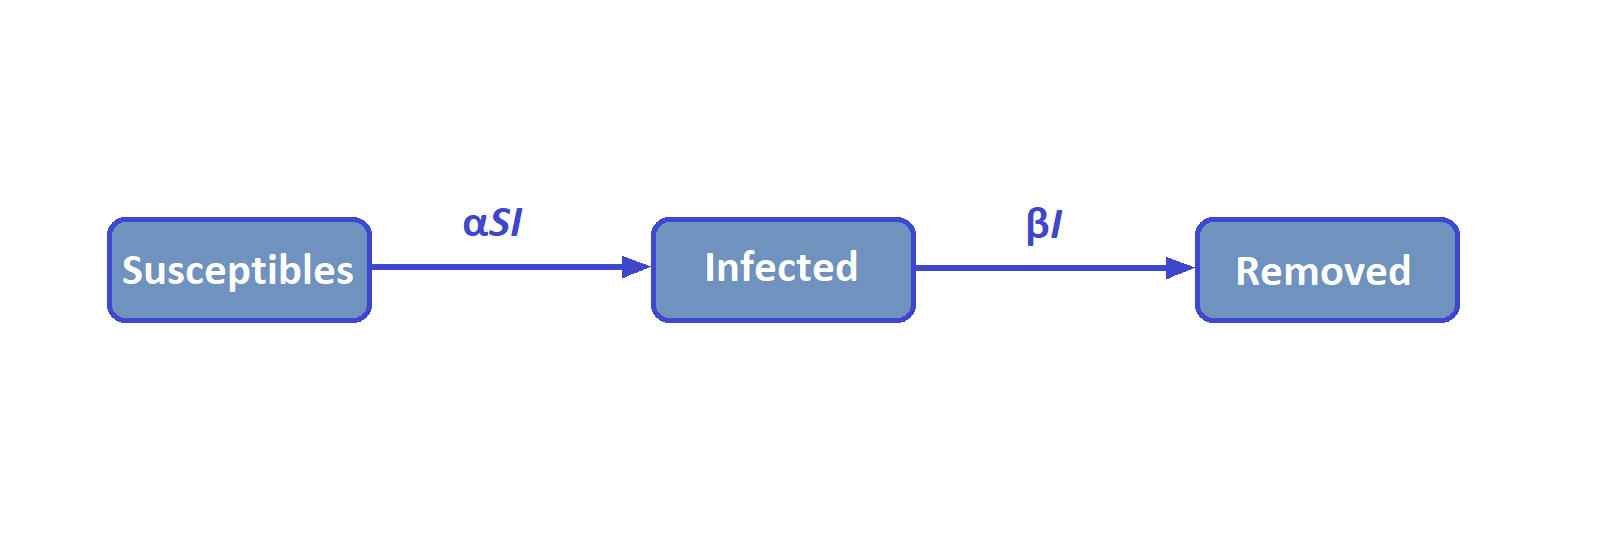
\includegraphics[width=0.75\textwidth]{./figures/SIR.png}
		\caption{Illustration of the population flow in the SIR model. S represents the ``Susceptible'', I
			the ``Infected'' and R the ``Removed'' population. The variable $\beta$ can also be redefined
			as $\frac{1}{b}$, where $b$ is the average duration of contagiousness}
		\label{fig:SIR}
	\end{center}
\end{figure}


\begin{align}
	\label{eq:SIR1}
	\frac{dS}{dt} &= -\alpha S I \\
	\frac{dI}{dt} &= \alpha S I - \beta I \\
	\frac{dR}{dt} &= \beta I
\end{align}


The model also assumes that the total number of individuals in the system $N$ remains constant in every time step and
that the sum of all transitions between all three groups during every time step remains zero\cite{kermack1991contributions}. This is expressed in the equations below.
$S(t)$, $I(t)$ and $R(t)$ express the number of individuals in each of the groups at time $t$, respectively.

\begin{align}
	\label{eq:SIR2}
	I(t) + S(t) + R(t) &= N \\
	\frac{dS}{dt} + \frac{dI}{dt} + \frac{dR}{dt} &= 0
\end{align}


Since the model assumes that the total population remains stable, phenomena like immigration, emigration or child birth are not accounted
for. While this does not correctly represent the real-world, it is assumed, that population fluctuations
due to these occurrences are minor enough compared to the entirety of a region's population that the assumption holds.\newline


In order to model the dynamics of an epidemic correctly, the variables of these differential
equations (like $\alpha$ and $\beta$ in this case) must be determined. This is part of solving the differential equations.
Different methods can be applied to achieve this goal. Two of these techniques are the \hyperref[sec:Gauss]{Gauss-Newton algorithm}
and \hyperref[sec:PSO]{Particle Swarm Optimization (PSO)}. Both of these techniques were used in this work and are explained
later in this chapter.


%-----------------------------------
%	SUBSECTION 3
%-----------------------------------
\subsection{The SEIRD model}
\label{sec:SEIRD}
The SEIRD model is a variant of the simpler SIR model\cite{knodel20173d} and aims to improve upon its predecessor by
introducing two new groups of individuals. These groups are used to differentiate the mechanics of an epidemic much
more precisely.
\textcolor{red}{(double check citation)}. % note
The five groups of the SEIRD model are shown below.

\begin{enumerate}[label=$\bullet$]
	\item \B{Susceptibles (S)}: Individuals that are not immune to the infection.
	\item \B{Exposed (E)}: Individuals that are infected, but show no or very little symptoms. These individuals
		do not quarantine yet and are therefor contributing to the spread of the disease.
	\item \B{Infected (I)}: Individuals that are severely sick and therefor hospitalized.
	\item \B{Recovered (R)}: Individuals that  have overcome the infection and are now immune to the disease.
	\item \B{Diseased (D)}: Individuals that have succumb to the infection.
\end{enumerate}


As described in the previous section, the transition between the individuals of different groups is the core
part of the model. The modified equations are shown below.

\begin{align}
	%\label{eq:SEIRD1}
	\frac{dS}{dt} &= -\alpha S E \label{eq:SEIRD1_S} \\
	\frac{dE}{dt} &= \alpha S E -\frac{1}{q} E \label{eq:SEIRD1_E} \\
	\frac{dI}{dt} &= \frac{\kappa}{q} E - \frac{1}{p} I \label{eq:SEIRD1_I} \\
	\frac{dR}{dt} &= \frac{1-\kappa}{q} E + \frac{1-\tau}{p} I \label{eq:SEIRD1_R} \\
	\frac{dD}{dt} &= \frac{\tau}{p} I \label{eq:SEIRD1_D} 
\end{align}

The transition between the \B{S} and \B{E} population in SEIRD is equivalent to the transition
between \B{S} and \B{I} in SIR. However, the population outflow from \B{E} is split and can either move
to \B{I} or \B{R}. This allows the modeling of infections that end in a quick recovery or an infection
with complications (defined as patient hospitalization). The ratio between the two scenarios is governed by the variable
$\kappa$. In addition, the variable $q$ was introduced and now represents the average duration until recovery/hospitalization of an
infected individual occurs. Similarly, the outflow of \B{I} is split between the populations of \B{R} and \B{D}. The ratio is governed
by the variable $\tau$. The equations for \B{R} and \B{D} were also adjusted to represent this change. Lastly, the variable $p$ was
introduced, which now represents the average stay of a hospitalized individual until they either recover or succumb to the infection.
\hyperref[fig:SEIRD]{Figure \ref*{fig:SEIRD}} illustrates all these changes.\\

\begin{figure}
	\begin{center}
		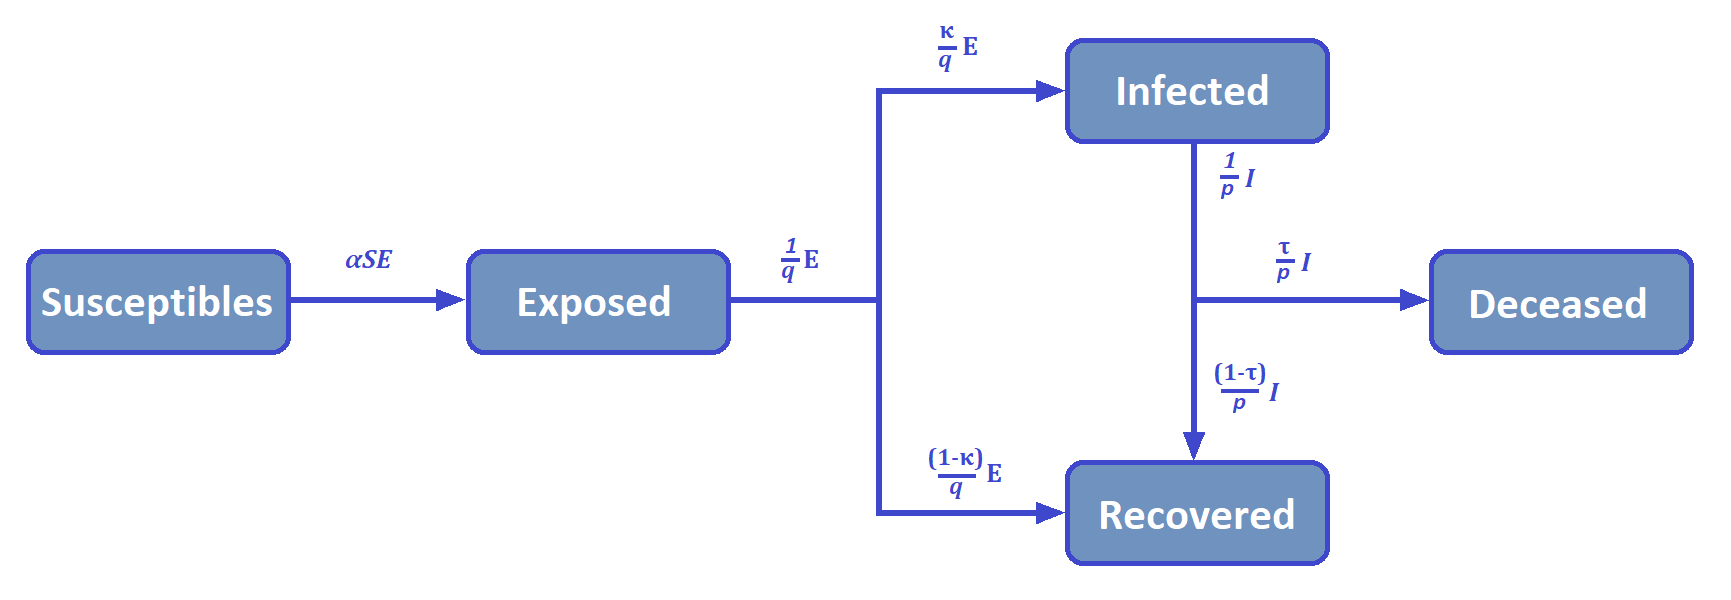
\includegraphics[width=0.75\textwidth]{./figures/SEIRD.png}
		\caption{Illustration of the population flow in the SEIRD model. S represents the ``Susceptible'', E the ``Exposed'',
			I the ``Infected'', R the ``Recovered'' and D the ``Diseased'' population.}
		\label{fig:SEIRD}
	\end{center}
\end{figure}



Like SIR, the SEIRD model assumes that the total number of individuals $N$ in the population remains constant during every step
of the modeling process. This leads to the equations expressed below. Again, $S(t)$, $E(t)$, $I(t)$, $R(t)$ and $D(t)$ express
the number of individuals for each group at time $t$, respectively. $N$ remains the total number of individuals in the model.

\begin{align}
	\label{eq:SEIRD2}
	S(t) + E(t) + I(t) + R(t) + D(t) &= N \\
	\frac{dS}{dt} + \frac{dE}{dt}  + \frac{dI}{dt} + \frac{dR}{dt} + \frac{dD}{dt} = 0
\end{align}


A model like this expresses the dynamics of an epidemic in greater detail. While the SIR model distinguishes between
groups like Susceptible and Infected, it does not differentiate between infected and hospitalized populations. This simplification
makes the modeling process easier but ignores real-world influences that could change the outcome of the simulation.
The SEIRD introduces these groups and aims to simulate a scenario that is much closer to the real-world.\newline

\textcolor{red}{move to methods?}\\
This work focused on the modeling capability of SEIRD in the transition stage between susceptibles and exposed. To fulfill this
task, the model was modified to better express phenomena specific to the COVID-19 pandemic. These changes are described in detail
in \hyperref[sec:SEIRDredef]{chapter~\ref*{chap:methodology}, section~\ref*{sec:SEIRDredef}}.


%----------------------------------------------------------------------------------------
%	SECTION 3
%----------------------------------------------------------------------------------------
\section{Variable optimization algorithms}
In order for the presented model equations to work properly, it is important to determine the correct value for each unknown variable.
Different methods to solve differential equations, but in the context of this work, the Gauss-Newton and the Particle Swarm Optimization (PSO)
algorithms were used. The following sections will explain the theory behind the two methods.


%-----------------------------------
%	SUBSECTION 1
%-----------------------------------
\subsection{Gauss-Newton algorithm}
\textcolor{red}{add citations, explain least squares better/at all}
\textcolor{red}{describe efficiency and why it is cool}
\label{sec:Gauss}
The \I{Gauss-Newton algorithm} is an iterative method that is used to solve non-linear least squares problems. Iterative means that the algorithm 
starts with an initial solution and tries to improve this solution successively over a number of consecutive steps.
Given a set of $m$ functions, $n$ variables that need to be optimized, a number of target values and a number of starting values, the algorithm tries
to optimize the variables in such a way that the difference between function results and target values is minimized.
The relevant parameters of this algorithm are shown below. 

\begin{align}
	F(\theta) =& (f_0(\theta), f_1(\theta),...,f_m(\theta))^T \\
	\theta^{i} =& (\theta^{i}_0, \theta^{i}_1, \theta^{i}_2,...,\theta^{i}_n)^T \\
	\epsilon^{i} =& F(\theta^{i}) - T \\
	\Delta^{i} =& (\theta^{i}_0 - \theta^{i-1}_0, \theta^{i}_1 - \theta^{i-1}_1, ..., \theta^{i}_m - \theta^{i-1}_m)^T %questionable?
\end{align}

$F(\theta)$ is the vector function, which contains $m$ functions and is
used to estimate the target values. $\theta^i$ is a vector of $n$ estimated input variables in iteration $i$, given to $F(\theta)$.
$\epsilon^i$ expresses the error between the estimation results and the vector of target values $T$ in iteration $i$.
$\Delta^i$ is the vector of adjustment values that are applied to the estimates of  iteration $i-1$, in order to improve the results of iteration $i$.
For the \I{Gauss-Newton algorithm} to be applicable, the condition $m > n$ must be satisfied.\newline

$F(\theta)$ is calculated iteratively thought the algorithm and can be expressed in the form of a Taylor Series, as shown in
\hyperref[eq:taylor1]{equation \ref*{eq:taylor1}}. It can then be rewritten to contain the Jacobian matrix $J$.

%note maybe add colors later
\begin{align}
	F(\theta^{i+1}) = F(\theta^{i} + \Delta^{i}) =&
		\begin{pmatrix} f_0(\theta^{i}) &+& \frac{\delta f_0(\theta)}{\delta \theta_0} \Delta^{i}_0 &+& ... &+&  \frac{\delta f_0(\theta)}{\delta \theta_n} \Delta^{i}_n  \\
				. && && && . \\
				. && && && . \\
				f_m(\theta^{i}) &+& \frac{\delta f_0(\theta)}{\delta \theta_0} \Delta^{i}_0 &+& ... &+&  \frac{\delta f_m(\theta)}{\delta \theta_n} \Delta^{i}_n 
		\end{pmatrix} \label{eq:taylor1} \\
	=& \begin{pmatrix} f_0(\theta^{i}) \\ . \\ . \\ f_m(\theta^{i})  \end{pmatrix} +
		\begin{pmatrix} \frac{\delta f_0(\theta)}{\delta \theta_0} & . & . & \frac{\delta f_0(\theta)}{\delta \theta_n}  \\
					   . &&& . \\
					   . &&& . \\
					   \frac{\delta f_m(\theta)}{\delta \theta_0} & . & . & \frac{\delta f_m(\theta)}{\delta \theta_n}
		\end{pmatrix} \begin{pmatrix} \Delta^{i}_0 \\ . \\ . \\ \Delta^{i}_n \end{pmatrix}  \label{eq:taylor2} \\
	=& F(\theta^{i}) + J \Delta^{i} \label{eq:taylor3}
\end{align}

	This means the Jacobian Matrix $J$ is defined as shown in \hyperref[eq:jacob]{equation \ref*{eq:jacob}}.

\begin{align}
	J_{pq} = \frac{\delta f_p(\theta)}{\delta \theta_q} \quad \text{where } \quad p \in \{0,1,..,m\},\text{ } q \in \{0,1,...,n\} \label{eq:jacob}
\end{align}

To minimize the error $\epsilon$ in each subsequent iteration, a connection is established between the current error and the
error of the following iteration. This process is shown below.

\begin{align}
	& \epsilon^{i+1} = F(\theta^{i} + \Delta^{i}) - T, \quad \text{since} \quad F(\theta^{i} + \Delta^{i}) = F(\theta^{i}) + J \Delta^{i} \\
	\Leftrightarrow & \epsilon^{i+1} = F(\theta^{i}) + J \Delta^{i} - T, \quad \text{since} \quad \epsilon^{i} = F(\theta^{i}) - T \\
	\Leftrightarrow & \epsilon^{i+1} = \epsilon^{i} + J \Delta^{i} \label{eq:taylor4}
\end{align}

\textcolor{red}{put equation in table format?}\\
$\epsilon^{i+1}$ is set to zero, since the goal of the algorithm is to minimize the error of the following iteration. Equation \ref*{eq:taylor4}
is then reorganized to take the form of a linear equation $Ax~=~b$. Since $\Delta$ steps usually are sufficiently small, it is assumed that the function is locally
	linear. This means that least squares analysis can be applied and used to rewrite equation \ref*{eq:taylor5} as shown below.

\begin{align}
	&\text{min} \| \epsilon^{i} + J \Delta^{i} \|\text{ over $\Delta^{i}$} \\
	\Rightarrow & \epsilon^{i} + J \Delta^{i} = 0 \qquad \text{rewrite to form $Ax = b$} \\
	\Leftrightarrow & J \Delta^{i} = -\epsilon^{i} \qquad \text{least squares: } x = (A^T A)^{-1} A^T b \label{eq:taylor5} \\
	\Leftrightarrow & \Delta^{i} = - (J^T J)^{-1} J^T \epsilon^{i} \label{eq:taylor6}
\end{align}

Hence, equation \ref*{eq:taylor6} can be used to calculate a suitable $\Delta$ to decrease the error in each subsequent iteration.\newline

A simplified \I{Gauss-Newton algorithm} is listed below as pseudo-code.

\begin{algorithm}
	\caption{\I{Gauss-Newton algorithm} pseudocode}
	\begin{algorithmic}
		\State Set $T$ = target values;
		\State Set $\theta^{0}$ = initial estimate for optimal varialbes;
		\State Calculate initial error $\epsilon^0$ = $F(\theta^0) - T$;
		\State Set i=0;
		\While {\{$\epsilon^i$ != 0 \B{or} (breaking conditions \B{not} fulfilled)\}}
			\State Calculate the Jacobian-Matrix $J$ using $\theta^i$;
			\State Calculate $J^{T}$ and  $(J^{T}J)^{-1}$;
			\State Use $\epsilon^i$, $J^{T}$ and  $(J^{T}J)^{-1}$ to calculate estimate adjustment $\Delta^i$;
			\State Set $\theta^{i}$ = $\theta^{i} + \Delta^i$;
			\State Set i = i+1;
			\State Calculate $\epsilon^i$;
		\EndWhile;
		\State \B{return} $\theta^i$;
	\end{algorithmic}
\end{algorithm}


%-----------------------------------
%	SUBSECTION 2
%-----------------------------------

\subsection{Particle Swarm Optimization}
\label{sec:PSO}
\textcolor{red}{double check PSO citation}
Like the Gauss-Newton algorithm, \I{Particle Swarm Optimization} (PSO) is an algorithm used to optimize a problem iteratively\cite{akman2018parameter}.
Generally, during PSO the following steps take place.

\begin{enumerate}
	\item Generate a number of candidate solutions (particles) per iteration
	\item Quantify the quality of each solution based on a chosen Loss function $L$
	\item Take the best candidate of the sum of all particles (swarm) as the current best solution
	\item If the best solution does not satisfy a chosen error margin and the number of iterations do not exceed a chosen
		maximum, repeat the previous steps
\end{enumerate}

%The general
%concept of PSO is to generate a number of candidate solutions (particles) per iteration, quantify the quality of each solution, take the best
%candidate of the sum of all particles (swarm) as the current best solution and try to improve this solution in following iterations.
%Improvements are made by randomly altering the candidate solutions in hopes of finding a new solution, that improves on the previous best.
%If suitable breaking conditions are met or the maximum number of iterations has passed, the algorithm stops and returns the current best solution.
%\newline

In order to find the best solution in a defined search space as quickly and efficiently as possible, additional conditions are usually applied
to each particle. Particles are grouped together, and a best group solution is set in each iteration, in addition to the global optimal solution.
Modifications of particle solutions in each iteration are random but in some way biased towards both the group and global optimum.
This is meant to direct a greater number of particles to the areas with the most optimal solutions, that are currently known.
However, these solutions may not be the global optimum for the defined search space, and there is no guarantee that any improvements are made during
an iteration. As a trade off, the problem function does not need to be differentiable like it is the case for the \I{Gauss-Newton algorithm}. \newline

During the initial steps of PSO, a problem space is defined as well as a loss function $L$. $L$ takes a number of $n$ input values in the from of a
vector $\theta$ and projects them to a real number $\epsilon$. The goal is to minimize the loss $L$ by optimizing $\theta$.
Written below is an exemplary PSO algorithm in  pseudocode.

\begin{algorithm}
	\caption{Particle Swarm Optimization pseudocode}
	\begin{algorithmic}
		\State Define Loss function $L(\theta)$;
		\State Define space of acceptable solutions;
		\State Set $\theta_S$ = uniformly chosen, random global solution;
		\State Set $G, P$ = number of groups, number of particles;
		\For {each element $j \in  \{0,1,...,G\}$}
			\State Initialize group;
			\State Initialize uniformly chosen, random solution $\theta_{g_j}$ for group;
			\If {$L(\theta_{g_j}) < L(\theta_S)$}
				\State Set $\theta_S$ = $\theta_{g_j}$;
			\EndIf
		\EndFor
		%\State Set P = number of paricles;
		\For {each element $i \in \{0,1,...,P\}$}
			\State Initialize a particle and set random particle solution $\theta_{p_i}$;
			\State Initialize group index $q$ = of one of the groups;
			\If {$L(\theta_{p_i}) < L(\theta_S)$}
				\State Set $\theta_S$ = $\theta_{p_i}$ and $g_q$ = $\theta_{p_i}$;
			\ElsIf {$L(\theta_{p_i}) < L(\theta_{g_q})$}
				\State Set $\theta_{g_q}$ = $\theta_{p_i}$;
			\EndIf
		\EndFor
		\While {$L(\theta_S) != 0$ \B{or} (breaking conditions are \B{not} met)}
			\For {each particle $i$}
				\State Modify solution $\theta_{p_i}$ (biased by $\theta_S$ and $\theta_{g_q}$);
				\If {$L(\theta_{p_i}) < L(\theta_S)$}
					\State Set $\theta_S$ = $\theta_{p_i}$ and $g_q$ = $\theta_{p_i}$;
				\ElsIf {$L(\theta_{p_i}) < L(\theta_{g_q})$}
					\State Set $\theta_{g_q}$ = $\theta_{p_i}$;
				\EndIf
			\EndFor
		\EndWhile
		\State \B{return} $\theta_S$;
	\end{algorithmic}
\end{algorithm}

